
\section{Geometría euclídea (del 25/01 al final)}

Llamamos geometría euclídea al espacio en el que podemos medir, cosa que hasta ahora no era posible.

Todo surge desde el módulo de un vector. Llamamos \concept[Módulo de un vector]{módulo de un vector} a la longitud que tiene. Dado $\vec{v}$, se define el módulo como $|\vec{v}|$.

\subsection{Producto, escalar, vectorial y mixto}

\paragraph{Introducción sobre el origen del producto escalar y vectorial}

Fuentes consultadas:
\begin{itemize}
  \item \href{http://www.suitcaseofdreams.net/Geometric_multiplication.htm}{Relación forma polar y binómica del producto complejo}
  \vspace{-0.4cm}
  \item \href{https://www2.clarku.edu/faculty/djoyce/complex/mult.html}{Interpretación geométrica del producto complejo}
  \vspace{-0.4cm}
  \item \href{https://www.quora.com/Who-invented-the-dot-product-and-cross-product}{Historia y aplicación de los cuaterniones los productos}
  \vspace{-0.4cm}
  \item \href{https://es.wikipedia.org/wiki/Cuaterni%C3%B3n}{ Extensión de los complejos al grupo de los quaterniones}
\end{itemize}

Dados 2 números complejos $z_1 = a_1+b_1i$, $z_2 = a_2+b_2i$. Expresando estos números complejos en forma polar tenemos: $z_1=r_{\alpha_1}$ y $z_2 = s_{\alpha_2}$.  

$z_1·z_2 = (a_1a_2 - b_1b_2) + (a_1b_2+a_2b_1)i = r·s_{\alpha_1+\alpha_2}$.

Tomando $z_1·\bar{z_2} = (a_1a_2 + b_1b_2) + (a_1b_2-a_2b_1)i = r·s_{\alpha_1-\alpha_2}
$

\subparagraph{Estudio de la parte real (producto escalar)}

En $Re(z_1·\bar{z_2}) = a_1a_2 + b_1b_2 = Re(r·s_{\alpha_1-\alpha_2})$

Para calcular $Re(r·s_{\alpha_1-\alpha_2}) = Re(r·s·\cos(\alpha_1-\alpha_2) + i·r·s·\sen(\alpha_1-\alpha_2)$, por lo que podemos completar:

$ a_1a_2 + b_1b_2 = |z_1||z_2|·\cos(\alpha_1-\alpha_2)$, y, siendo conscientes que $\alpha_1-\alpha_2$ es el ángulo que forman los 2 vectores, obtenemos la expresión del producto escalar de 2 vectores.


\subparagraph{Estudio de la parte imaginaria (producto vectorial)}

Al extender este razonamiento al grupo de los cuaterniones, tendríamos:

\newcommand{\quat}{\vec}

$Re(z_1\bar{z_2}) = Re\left((b_1\quat{i}+c_1\quat{j}+d_1\quat{k})·(-b_2\quat{i}-c_2\quat{j}-d_2\quat{k})\right) = (b_1b_2+c_1c_2+d_1d_2)$

Lo espectacular viene al considerar la parte "imaginaria" (aunque no tengamos claro cómo se define ese concepto en los cuaterniones):

$Im(z_1\bar{z_2}) = f(\quat{i},\quat{j},\quat{k})$, cuya expresión analítica es la del producto vectorial, ya que en grupo de los cuaterniones $\quat{i}\quat{j}=\quat{k}$ y todo eso.

\subsubsection{Producto escalar}

\begin{itemize}
  \item Definición.
  \item Base ortogonal y ortonormal.
  \item Expresión analítica.
  \item Cálculo del módulo (porque Pitágoras tridimensional no funciona).
  \item Base canónica.
  \item Interpretación geométrica (proyección).
\end{itemize}

\subsubsection{Producto vectorial}
\begin{itemize}
  \item Definición.
  \subitem Regla de la mano derecha
  \item Expresión analítica.
  \item Interpretación geométrica. 
\end{itemize}


\subsubsection{Producto mixto}

\begin{itemize}
  \item ¿Qué ocurre si en el producto vectorial meto un vector en lugar de $\vec{i},\vec{j},\vec{k}$?
  \item Definición.
  \item Expresión analítica.
  \item Interpretación geométrica. 
\end{itemize}

\subsubsection{Practicamos en general ejercicios del tema 9}

\subsection{Aplicación de los productos}

\subsubsection{Vector normal del plano}

\subsubsection{Vector director de la recta en implícitas}

\begin{figure}[hbtp]
\centering
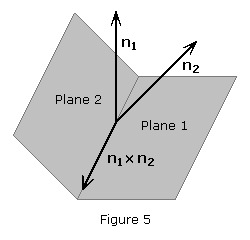
\includegraphics{img/directorrectaimplicitas.jpg}
\end{figure}

Dada una recta $r$ que pertenece a ambos planos, $\pi_1$ y $\pi_2$, $\vec{V_r}\perp n_{\pi_1} \wedge \vec{V_r}\perp n_{\pi_2}$. Por eso, para buscar un vector perpendicular a la vez a 2 vectores dados, el camino más corto es el producto vectorial.

$\vec{V_r} = n_{\pi_1}\times n_{\pi_2}$

\begin{problem}

Halla la recta perpendicular a $r:\frac{x-1}{2} = \frac{y+2}{3} = \frac{2z-2}{3}$ que pasa por el punto $P(1,-2,0)$.

\solution

La recta pedida es $t:\left\{\begin{array}{c}P\in t\\t\perp r\\\end{array}\right.$ 

Todas las rectas perpendiculares a una recta forman un plano. Llamamos $\pi$ a ese plano. Así, $ t \in \pi, \text{ con } \pi:\left\{\begin{array}{c}P\in\pi\\\pi\perp r\end{array}\right.$. Así, $t$ será la recta determinada por $A = t\cap\pi, P(1,-2,0)$

$\pi\perp r\implies n_{\pi} || \vec{V_r}$. Tomamos $n_{\pi}  = \left(2,3,\rfrac{3}{2}\right)$

Como $P\in\pi\implies 2P_1 + 3P_2 +\rfrac{3}{2}P_3 + D = 0 \dimplies 2-6+D = 0 \dimplies D=4$

Así, $\pi: 2x+3y+\rfrac{3}{2}z + 4 = 0$

2) Buscamos $A=\pi\cap r$. Tendremos $t:\{A,P\}$


\[
  \left\{\begin{array}{c}
    2x+3y+\rfrac{3}{2}z + 4 = 0\\
    x = 1 + 2\lambda\\
    y = -2 + 3\lambda\\
    z = 1 + \rfrac{3}{2}\lambda\end{array}\right\} \implies 2+4\lambda - 6 + 9\lambda + \rfrac{3}{2} + \rfrac{9}{4}\lambda + 4 = 0 \dimplies 
\]
\[
  \frac{3}{2}+\left(13+\rfrac{9}{4}\right)\lambda = 0 \dimplies \lambda = \frac{\rfrac{61}{4}}{\rfrac{3}{2}} = \frac{61}{6}
\]

Sustituimos $\lambda$ en la ecuación de la recta para obtener $A$:
$\left\{\begin{array}{c}
    x = 1 + 2\rfrac{61}{6} = \frac{64}{3}\\
    y = -2 + 3\rfrac{61}{6} = \frac{57}{2}\\
    z = 1 + \rfrac{3}{2}\rfrac{61}{6} = \frac{57}{4}
\end{array}\right\}$


\[A = \pi\cap r = \left(\frac{64}{3},\frac{57}{2},\frac{57}{4}\right)\]

3) Buscamos la recta $r$ que pasa por los puntos $A$ y $P$. 

$\vec{AP} = \left(\frac{64}{3}-1,\frac{57}{2}+2,\frac{57}{4}\right) =  \left(\frac{61}{3},\frac{61}{2},\frac{57}{4}\right)$

\[r : \{A,\vec{V_r}\} = \left\{\begin{array}{c}
    x = \rfrac{64}{3} + 2\lambda\\
    y = \rfrac{57}{2} + 3\lambda\\
    z = \rfrac{57}{4} + \rfrac{3}{2}\lambda
\end{array}\right\}\]

\end{problem}

127,128.

\begin{problem}[Junio 2019]

Dados los puntos $A(1,1,1), B(1,3,-3)$ y $C(-3,-1,1)$, se pide:
\ppart Determinar la ecuación del plano que contiene a los 3 puntos.
\ppart Obtener un punto $D$ (distinto a los anteriores) tal que los vectores $\vec{AB}$, $\vec{AC}$,$\vec{AD}$ sean linealmente dependientes.
\ppart Encontrar un punto $P$ del eje $OX$, de modo que el volumen del tetraedro de vértices $A$,$B$,$C$,$P$ sea igual a 1.

\solution

\spart 

Tomamos $\vec{AB} = (0,2,-4)$, $\vec{AC} = (-4,-2,0)$ como vectores directores del plano y calculamos su ecuación implícita:

\[
\pi: \left|\begin{array}{ccc}
x - 1 & 0 & -4\\
y - 1 & 2 & -2\\
z - 1 & -4& 0
\end{array}\right| = 0 \dimplies 16y-16 + 8z-8-8x+8 = 0\]
\[\dimplies -8x + 16y + 8z -16 = 0 \dimplies -x+2y+z-2=0
\]

\spart Basta con tomar $D\in\pi$. Por ejemplo: $D(0,1,0)\in\pi$.

Comprobamos que $\vec{AB},\vec{AC},\vec{AD}$ son linealmente dependientes calculando el determinante de la matriz que forman.

$\vec{AD} = (1,0,1)$

\[
|\vec{AB}\quad\vec{AC}\quad\vec{AD}| = 
\left|\begin{array}{ccc}
1 & 0 & -4\\
0 & 2 & -2\\
1 & -4& 0
\end{array}\right| = 0
\]

\spart 

(Ojo que aquí no se puede simplificar, aunque antes sí hubiéramos podido)

El volumen del tetraedro será $\rfrac{1}{6}$ del voluen del paralelepípedo:

\[
||\vec{AB}\quad\vec{AC}\quad\vec{AD}|| = 
\left|\left|\begin{array}{ccc}
1 & 0 & -4\\
1 & 2 & -2\\
a-1 & -4& 0
\end{array}\right|\right| = 2·2·\left|\left|\begin{array}{ccc}
1 & 0 & 2\\
1 & 1 & 1\\
z-1 & -2& 0
\end{array}\right|\right| = {6} 
\]
\[
 \left|\left|\begin{array}{ccc}
1 & 0 & 2\\
1 & 1 & 1\\
a-1 & -2& 0
\end{array}\right|\right| = \frac{3}{2}  \dimplies
|-4 -2a-2+2| = \frac{3}{2}\dimplies |-4-2a| = \rfrac{3}{2} \implies\]
\[
\left\{\begin{array}{c}
-4-2a_1 = \rfrac{3}{2} \dimplies a_1 = \frac{-11}{4} \to P_1\left(\rfrac{-11}{4},0,0\right)\\
4+2a_2 = \rfrac{3}{2} \dimplies a_2 = \frac{-5}{4} \to P_2\left(\rfrac{-5}{4},0,0\right)
\end{array}\right.
\]

\end{problem}


\subsection{Proyecciones y simetrías (Libro)}

\subsubsection{Proyección}

\paragraph{Proyección de punto sobre plano}
\index{Proyección!punto sobre plano}

Para calcular la proyección de un punto $P$ sobre un plano $\pi$ (ver \fref{fig::proy::punto-plano}):
\begin{enumerate}
  \item $r\perp \pi$ con $P\in r$
  \item $P' = r\cap \pi$
\end{enumerate}

\begin{figure}[hbtp]
\centering
\tdplotsetmaincoords{60}{110}

\begin{tikzpicture}[tdplot_main_coords,scale=0.8]
    % draw axes
    \fill[blue!20!white] (-2,-2,0) to (5,-2,0) to (5,5,0) node[anchor=south,color=black]{$\pi$} to (-2,5,0)to cycle;
    \draw[dashed,color=black!45!white] (2,2,-1) -- (2,2,4) node[anchor=west]{$r\perp\pi$};
    \draw[fill] (2,2,3) circle(1pt) node[anchor=west]{$P$};
    \draw[fill,color=red] (2,2,0) circle(1pt) node[anchor=west]{$P'$};
\end{tikzpicture}
\label{fig::proy::punto-plano}
\caption{Proyección de punto sobre plano}
\end{figure}

\paragraph{Proyección de recta sobre plano}
\index{Proyección!recta sobre plano}

Se reduce a proyectar 2 puntos de la recta sobre el plano. Se puede utilizar el punto de intersección de la recta con el plano.

\obs Buenas prácticas: calcular el punto de intersección para saber si la recta pertenece al plano o es paralela. 
\begin{itemize}
  \item Si $r\in\pi$, la proyección de la recta será ella misma.
  \item Si $r||\pi$, necesitaremos proyectar 2 puntos de la recta.
  \item En los demás casos, se proyecta un punto sobre la recta y la proyección será la que pasa por el punto proyectado y el punto de intersección. Ver \fref{fig::proy::recta-plano}.
\end{itemize}


\begin{figure}[hbtp]
\centering
\tdplotsetmaincoords{60}{110}
\begin{tikzpicture}[tdplot_main_coords,scale=0.8]
    % draw axes
    \fill[blue!20!white] (-2,-2,0) to (6,-2,0) to (6,6,0) node[anchor=south,color=black]{$\pi$} to (-2,6,0)to cycle;
    \draw (0,0,0) -- (2.5,5,5) node[anchor=west]{$r$};
    \draw[dashed] (-1,-2,-2) -- (0,0,0);
    \draw[fill] (0,0,0)circle(2pt) node[anchor=south]{$Q$};
    \draw[fill] (2,4,4)circle(2pt) node[anchor=north west]{$P$};
    \draw[fill] (2,4,0) circle(2pt) node[anchor=north]{$P'$};
    \draw[dashed] (2,4,4) -- (2,4,0);
    \draw[color=red] (-1,-2,0) -- (2.5,5,0) node[anchor=north east]{$r'$};  
\end{tikzpicture}
\label{fig::proy::recta-plano}
\caption{Proyección de recta sobre plano}
\end{figure}


\paragraph{Proyección de punto sobre recta}
\index{Proyección!punto sobre recta}

\begin{figure}[hbtp]
\centering
\tdplotsetmaincoords{60}{110}
\begin{tikzpicture}[tdplot_main_coords,scale=0.8]
    % draw axes
    \fill[blue!20!white] (-4,0,-2) to (4,0,-2) to (4,0,4) node[anchor=south,color=black]{$\pi$} to (-4,0,4)to cycle;
    \draw (0,0,0) -- (0,4,0) node[anchor=east]{$r$};
    \draw[dashed] (0,-1.6,0) -- (0,0,0);
    \draw (0,-1.6,0)--(0,-3,0);
    \draw[fill,color=red] (0,0,0)circle(2pt) node[anchor=north]{$P'$};
    \draw[fill] (0,0,3)circle(2pt) node[anchor=west]{$P$};
    \draw[dashed] (0,0,0) -- (0,0,3);
\end{tikzpicture}
\label{fig::proy::punto-recta}
\caption{Proyección de punto sobre recta}
\end{figure}


\subsubsection{Simetría de un punto respecto de otro punto}

\index{Simetría!punto respecto de punto}

\begin{figure}[hbtp]
\centering
\tdplotsetmaincoords{60}{110}
\begin{tikzpicture}[tdplot_main_coords,scale=0.8]
    % draw axes
    %\fill[blue!20!white] (-2,-2,0) to (6,-2,0) to (6,6,0) node[anchor=south,color=black]{$\pi$} to (-2,6,0)to cycle;
    \draw[dashed] (0,3,0) -- (0,0,0);
    \draw[dashed] (0,-3,0) -- (0,3,0);
    \draw[fill,color=red] (0,-3,0)circle(2pt) node[anchor=south]{$P'$};
    \draw[fill] (0,3,0)circle(2pt) node[anchor=south]{$P$};
    \draw[fill] (0,0,0) circle(2pt) node[anchor=south]{$M_{PP'}$};
\end{tikzpicture}
\label{fig::sim::punto-punto}
\caption{Simetría de un punto respecto de otro punto}
\end{figure}

\subsubsection{Simetría de un punto respecto de una recta}
\index{Simetría!punto respecto de recta}

Plano perpendicular a la recta que contenga al punto, intersección con la recta.

\begin{figure}[hbtp]
\centering
\tdplotsetmaincoords{60}{110}
\begin{tikzpicture}[tdplot_main_coords,scale=0.8]
    % draw axes
    \fill[blue!20!white] (-4,0,-4) to (4,0,-4) to (4,0,4) node[anchor=south,color=black]{$\pi$} to (-4,0,4)to cycle;
    \draw (0,0,0) -- (0,4,0) node[anchor=east]{$r$};
    \draw[dashed] (0,-1.6,0) -- (0,0,0);
    \draw (0,-1.6,0)--(0,-3,0);
    
    \draw[fill] (0,0,2)circle(2pt) node[anchor=west]{$P$};
    \draw[fill] (0,0,0)circle(2pt) node[anchor=north]{$M_{PP'}$};
    \draw[fill,color=red] (0,0,-2)circle(2pt) node[anchor=west]{$P'$};
    \draw[dashed] (0,0,-2) -- (0,0,2);
\end{tikzpicture}
\label{fig::sim::punto-recta}
\caption{Simetría de punto respecto de recta}
\end{figure}


\subsubsection{Simetría de un punto respecto de un plano}
\index{Simetría!punto respecto de un plano}

Recta perpendicular al plano, que pasa por el punto.

\begin{figure}[hbtp]
\centering
\tdplotsetmaincoords{60}{110}
\begin{tikzpicture}[tdplot_main_coords,scale=0.8]
    % draw axes
    \fill[blue!20!white] (-2,-2,0) to (5,-2,0) to (5,5,0) node[anchor=south,color=black]{$\pi$} to (-2,5,0)to cycle;
    \draw(2,2,1) -- (2,2,3);
    \draw(2,2,0) -- (2,2,1) node[anchor=west]{$r\perp\pi$};
    \draw[dashed](2,2,-2) -- (2,2,0);
    \draw(2,2,-3) -- (2,2,-2);
    \draw[fill] (2,2,3)circle(1pt) node[anchor=east]{$P$};
    \draw[fill] (2,2,0) circle(1pt) node[anchor=north east]{$M_{PP'}$};
    \draw[fill,color=red] (2,2,-3) circle(1pt) node[anchor=east]{$P'$};
\end{tikzpicture}
\label{fig::sim::punto-plano}
\caption{Simétrico de punto respecto de un plano}
\end{figure}



\subsubsection{Simetría de una recta respecto de un plano}
\index{Simetría!recta respecto de plano}

\begin{figure}[hbtp]
\centering
\tdplotsetmaincoords{60}{110}

\begin{tikzpicture}[tdplot_main_coords,scale=0.8]
    % draw axes
    \fill[blue!20!white] (-2,-2,0) to (6,-2,0) to (6,6,0) node[anchor=south,color=black]{$\pi$} to (-2,6,0)to cycle;
    \draw (0,0,0) -- (2.5,5,5) node[anchor=east]{$r$};
    \draw[dashed] (-1,-2,-2) -- (0,0,0);
    \draw[fill] (0,0,0)circle(2pt) node[anchor=south]{$Q$};
    \draw[fill] (2,4,4)circle(2pt) node[anchor=north west]{$P$};
    \draw[fill] (2,4,0) circle(2pt) node[anchor=north]{$M_{PP'}$};
    \draw[fill] (2,4,-4) circle(2pt) node[anchor=north]{$P'$};
    \draw[dashed] (2,4,4) -- (2,4,-4);
    \draw[color=red] (-1,-2,2) -- (0,0,0);  
    \draw[color=red,dashed] (0,0,0) -- (1.4,2.8,-2.8) node[anchor=north east]{$r'$};  
    \draw[color=red] (1.4,2.8,-2.8) -- (2,4,-4) ;  
\end{tikzpicture}
\label{fig::sim::recta-plano}
\caption{Simetría de una recta respecto de un plano}
\end{figure}



\newpage
\subsection{Ángulos}
\subsubsection{Ángulo formado por dos rectas}
\index{Ángulo!formado por dos rectas}

Llamamos ángulo formado por 2 rectas al menor de los 2 ángulos que forman (en la \fref{fig::ang-recta-recta}, llamaríamos $\widehat{r,s} = \alpha$). Según su posición relativa se distinguen:

\begin{itemize}
  \item \textbf{Secantes:} el ángulo de las rectas será el ángulo de los vectores directores.
  \item \textbf{Paralelas/coincidentes:} ángulo 0.
  \item \textbf{Rectas que se cruzan:} el ángulo que forman es el que forman 2 paralelas a ellas que sean secantes. 
\end{itemize}

Se calcula el ángulo desde la definición de producto escalar.

\[
\cos(\alpha) = \cos(\hat{r,x}) = \left| \cos\left(\hat{\vec{u_r},\vec{v_r}}\right)\right| = \frac{|\vec{u_r}·\vec{v_r}|}{|\vec{u_r}|·|\vec{v_r}|} \implies 0\lq \alpha \leq \rfrac{\pi}{2}
\]


\begin{figure}[hbtp]
\centering
\tdplotsetmaincoords{60}{110}
\begin{tikzpicture}[scale=0.8]
    % draw axes
\coordinate (a) at (0,0);
\coordinate (b) at (3,2);
\coordinate (c) at (0,3);

\draw pic[draw,fill=green!30,angle radius=1cm,"$\beta$" shift={(15mm,1mm)}] {angle=c--a--b};
\draw pic[draw,fill=blue!30,angle radius=0.5cm,"$\alpha$" shift={(3mm,4mm)}] {angle=b--a--c};

\draw  (-3,-2) -- (a) -- node[above] {$r$} (b);
\draw  (0,-3) -- (a) -- node[above right] {$s$} (c);
\end{tikzpicture}
\label{fig::ang-recta-recta}
\caption{Ángulo formado por 2 rectas}
\end{figure}


\subsubsection{Ángulo formado por dos planos}
\index{Ángulo!formado por dos planos}

Llamamos ángulo formado por 2 planos al menor de los 2 ángulos diedros que forman 2 planos secantes.

\obs Si los planos son paralelos, no forman ningún ángulo.

\begin{figure}[hbtp]
\centering
\tdplotsetmaincoords{60}{110}
%\input{tikz/ang-plano-plano.tex}
\label{fig::ang-plano-plano}
\caption{Ángulo formado por 2 planos}
\end{figure}

\subsubsection{Ángulo formado por recta y plano}
\index{Ángulo!formado por recta y un plano}

\begin{itemize}
  \item Sería posible calcular el ángulo que forma la recta con su proyección. Ver \fref{fig::ang-recta-plano}.
  \item Otra posibilidad, utilizar el vector normal del plano.
\end{itemize}


\begin{figure}[hbtp]
\centering
\tdplotsetmaincoords{60}{110}
\begin{tikzpicture}[tdplot_main_coords,scale=0.8]
    % draw axes
    \coordinate (P) at (2,4,4);
    \coordinate (O) at (0,0,0);
    \coordinate (Q) at (2,4,0);

    % draw axes
    \fill[blue!20!white] (-2,-2,0) to (6,-2,0) to (6,6,0) node[anchor=south,color=black]{$\pi$} to (-2,6,0)to cycle;
    \draw (0,0,0) -- (2.5,5,5) node[anchor=east]{$r$};
    \draw[dashed] (-1,-2,-2) -- (0,0,0);
    \draw[fill] (0,0,0)circle(2pt) node[anchor=south]{$Q$};
    \draw[fill] (2,4,4)circle(2pt) node[anchor=north west]{$P$};
    \draw[fill] (2,4,0) circle(2pt) node[anchor=north]{$P_{\pi}$};
    
    \draw[dashed] (2,4,4) -- (2,4,0);


    \draw[color=red,dashed] (-1,-2,0) -- (0,0,0);  
    \draw[color=red,dashed] (0,0,0) -- (1.4,2.8,0) node[anchor=north east]{$r_{\pi}$};  
    \draw[color=red,dashed] (1.4,2.8,0) -- (2.5,5,0); 


    \pic [color=green!30!black,fill=green!30!black,draw, ->, "$\alpha$", angle eccentricity=1.5] {angle = Q--O--P};
    %\fill[color=green!30!black] (0,0,0) -- (-0.5,0,0) -- (-0.635,0.35,0) -- cycle;
\end{tikzpicture}
\label{fig::ang-recta-plano}
\caption{Ángulo formado por una recta y un plano}
\end{figure}

\begin{problem}

Calcula el ángulo formado por la recta $r$ y el plano $\pi$.

\[
r : \begin{cases} 2x-3y+z=0\\x-z=0\end{cases}\;\;\;\pi: x+y-2z=3
\]
\solution

Obtenemos las ecuaciones paramétricas de la recta, calculando las soluciones del sistema compatible indeterminado:

\[
r : \begin{cases} 2x-3y+z=0\\x-z=0\end{cases} \overset{x=\lambda}{\to}
\begin{cases} 2\lambda-3y+\lambda = 0 \to y=\lambda \\x=z=\lambda\end{cases} \dimplies \begin{cases}x=\lambda\\y=\lambda\\z=\lambda\end{cases}
\]

\ul{Método 1: Angulo entre vectores}

\[
\widehat{\pi,\vec{v_r}} = 90 - \widehat{\vec{n_{\pi}},\vec{v_r}}
\]

\[
\cos\left(\widehat{\vec{n_{\pi}},\vec{v_r}}\right) = \frac{|\vec{n_{\pi}}·\vec{v_r}|}{|\vec{n_{\pi}}|·|\vec{v_r}|} = \frac{(1,1,1)·(1,1,-2)}{\sqrt{1^2+1^2+1^2}·\sqrt{1^2+1^2+(-2)^2}} = 0 
\]

\[
\cos\left(\widehat{\vec{n_{\pi}},\vec{v_r}}\right) = 0\implies \widehat{\vec{n_{\pi}},\vec{v_r}} = 90 \implies \widehat{\pi,\vec{v_r}} = 0 \implies \pi|| r
\]


\ul{Método 2: Ángulo con la proyección}

Para calcular la proyección de una recta sobre un plano:
\begin{enumerate}
  \item Comprobamos $r\in \pi: \lambda+\lambda-2\lambda = 3 \nexists\lambda\in\real\implies r||\pi$ con $r\cap\pi=\emptyset$ 
  
  \item Varias opciones:
  \subitem a) Necesitamos proyectar 2 puntos de la recta sobre el plano. Tomamos los puntos $A(0,0,0)\in r$ y $B(1,1,1)\in r$.

  \textbf{$A_{\pi}$:} Calculamos $t\perp\pi (\implies \vec{v_t}||\vec{n_{\pi}})$ con $A\in t\to t\begin{cases}x=\lambda\\y=\lambda\\z=-2\lambda\end{cases}$

  Calculamos $t\cap\pi: \lambda+\lambda+4\lambda=3\dimplies \lambda=\rfrac{1}{2} \implies t\cap\pi =A_{\pi}=\left(\rfrac{1}{2},\rfrac{1}{2},-1\right)$

  \textbf{$B_{\pi}$:} Calculamos $t'\perp\pi (\implies \vec{v_t'}||\vec{n_{\pi}})$ con $B\in t'\to t'\begin{cases}x=1+\mu\\y=1+\mu\\z=1-2\mu\end{cases}$

  Calculamos $t'\cap\pi: (1+\mu)+(1+\mu)-2(1-2\mu)=3\dimplies \mu=\rfrac{1}{2} \implies t\cap\pi =B_{\pi}=\left(\rfrac{3}{2},\rfrac{3}{2},0\right)$

  Calculamos $r_{\pi}:\{A,\vec{AB}\} \dimplies r:\begin{cases}x=\rfrac{1}{2}+\lambda\\y=\rfrac{1}{2}+\lambda\\z=\rfrac{1}{2}+\lambda\end{cases}$

\obs ¿Es casualidad que $\vec{v_r} = \vec{v_{r_{\pi}}}$? No, una recta paralela a un plano y su proyección sobre ese plano son rectas paralelas, por lo que tienen vectores directores proporcionales.

\end{enumerate}

\end{problem}

\concept{Paralelismo y perpendicularidad entre recta y plano}

\begin{itemize}
  \item $r || \pi \dimplies \vec{v_r}·\vec{n_{\pi}} = 0$
  \item $r\perp \pi \dimplies \vec{v_r}||\vec{n_{\pi}}$
\end{itemize}

\subsection{Distancias}
\subsubsection{Entre 2 puntos}
Módulo del vector.

\subsubsection{Entre punto y plano}

La distancia entre el punto y su proyección sobre el plano. Ver \fref{fig::dist-punto-plano}.
\index{Distancia!punto-plano}


\begin{itemize}
  \item $d(P,\pi) = |PP_{\pi}|$, siendo $P_{\pi}$ la proyección del punto sobre el plano.
  \item Se puede utilizar otro camino más corto para calcular esta distancia. Ver \fref{fig::dist-punto-plano}.

  \subitem Consideramos $Q\in\pi$.
  \subitem $|\vec{n_{\pi}}·\vec{QP}| = |\vec{n_{\pi}}|·|\vec{QP}|·\cos(\alpha)$, siendo $\alpha$ el ángulo que forman estos vectores.
  \subitem Aplicando la definición de coseno: $\cos(\alpha) = \rfrac{d(P,\pi)}{|\vec{QP}|}$.
  \subitem Sustituyendo y despejando: $|\vec{n_{\pi}}·\vec{QP}| = |\vec{n_{\pi}}|·d(P,\pi) \to d(P,\pi) = \frac{|\vec{n_{\pi}}·\vec{QP}|}{|\vec{n_{\pi}}|}$
  \subitem $|\vec{n_{\pi}}·\vec{QP}| = |A(p_1-q_1) + B(p_2-q_2) + C(p_3-q_3)| = Ap_1+Bp_2+Cp_3+D$
  \subitem \textbf{Conclusión:}\index{Distancia! punto-plano}

  \[
    d(P,\pi) = \frac{|Aq_1+Bq_2+Cq_3+D|}{|(A,B,C)|}
  \]
\end{itemize}

\begin{figure}[hbtp]
\centering
\tdplotsetmaincoords{60}{110}
\begin{tikzpicture}[tdplot_main_coords,scale=0.8]
    % draw axes
    \fill[blue!20!white] (-2,-2,0) to (6,-2,0) to (6,6,0) node[anchor=south,color=black]{$\pi$} to (-2,6,0)to cycle;
    \draw[->] (0,0,0) -- (2,4,4) node[anchor=south east]{$\overset{\to}{PQ}$};
    \draw[fill] (0,0,0)circle(2pt) node[anchor=south]{$Q$};
    \draw[fill] (2,4,4)circle(2pt) node[anchor=north west]{$P$};
    \draw[fill] (2,4,0) circle(2pt) node[anchor=north]{$P_{\pi}$};
    \draw[->] (0,0,0) -- (2,4,0);
    \draw (1,2,0) node[anchor=north east]{$\overset{\to}{QP_{\pi}}$};
    \draw[dashed] (2,4,4) -- (2,4,0);
    \draw[->,color=red!50!black] (2,4,0) -- (2,4,2) node[anchor=west]{$n_{\pi}$};
\end{tikzpicture}
\label{fig::dist-punto-plano}
\caption{Distancia de un punto a un plano}
\end{figure}

\[d(P,\pi) = \frac{|Ap_1+Bp_2+Cp_3+D|}{|(A,B,C)|}\]

\subsubsection{Entre 2 planos o entre una recta y un plano}
\index{Distancia!plano-plano}
\index{Distancia!recta-plano}

\begin{itemize}
  \item Se comprueba si son paralelos (porque sino, distancia 0).
  \item Si no lo son, calculamos la distancia entre un punto que pertenezca al plano o a la recta y al otro plano.
\end{itemize}

\subsubsection{Entre punto y recta}
\index{Distancia!punto-recta}

\begin{itemize}
  \item $d(P,r) = |PP_{r}|$, siendo $P_r$ la proyección de $P$ sobre $r$.
  \item Otra manera de calcular sería considerar un punto $Q\in r$. Ver \fref{fig::dist-punto-recta}.
  \subitem Considerando $\vec{QP}$ y $\vec{v_r}$ (ambos fáciles de calcular), $d(P,r)$ se podría calcular utilizando la definición de seno. Así,
  
  \[\sen\left(\widehat{\vec{v_r},\vec{QP}}\right) = \displaystyle\frac{|d(P,r)|}{|\vec{QP}|}\]

  \subitem Utilizando $|\vec{QP}\times\vec{v_r}| = |\vec{QP}|·|\vec{v_r}|\sen(\alpha)$, despejamos:
  \[
    |\vec{QP}\times\vec{v_r}| = |\vec{QP}|·|\vec{v_r}|·\frac{|d(P,r)|}{|\vec{QP}|} \dimplies d(P,r) = \frac{|\vec{QP}\times\vec{v_r}|}{|\vec{v_r}|}
  \]
\end{itemize}

\begin{figure}[hbtp]
\centering
\tdplotsetmaincoords{60}{110}
\begin{tikzpicture}[scale=1.2]
    % draw axes
    \draw (-3,0) to (3,0) node[anchor=north]{$r$};
    \draw[fill] (-1,0)circle(1pt) node[anchor=south]{$Q$};

    \draw[fill] (1,0)circle(1pt) node[anchor=north west]{$P_{r}$};
    \draw[fill] (1,2)circle(1pt) node[anchor=west]{$P$};
    \draw[->] (-1,0) -- (0,0) node[anchor=north]{$\overset{\to}{v_r}$};
    \draw[->] (1,0) -- (1,2);
    \draw(1,1) node[anchor=west]{$d(P,r)$};
    \draw[->] (-1,0) -- (1,2);
    \draw(0,1.5) node{$\overset{\to}{PQ}$};
\end{tikzpicture}
\label{fig::dist-punto-recta}
\caption{Distancia de un punto a una recta}
\end{figure}



\subsubsection{Entre 2 rectas}
\index{Distancia!recta-recta}
\begin{itemize}
  \item Comprobamos si $r||s$. 
  \subitem Si $r||s \implies d(r,s) = d(P_r,s) = d(P_s,r)$
  \subitem Si $r\not|| s \implies d(r,s) = d(r,\pi)$, con $\pi:\{v_r,v_s,P_s\}$
\end{itemize}


\subsection{Lugares geométricos}
\subsubsection{Perpendicular común}
\subsubsection{Plano mediador}
\subsubsection{Planos bisectores}

\subsection{Áreas y volúmenes}
\begin{itemize}
  \item Área del paralelogramo: $\left|\vec{a}\times\vec{b}\right|$
  \item Área del triángulo: $\rfrac{1}{2}·\left|\vec{a}\times\vec{b}\right|$
  \item Volumen del paralelepípedo: $\left|[\vec{a},\vec{b},\vec{c}]\right|$
  \item Volumen del tetraedro: $\rfrac{1}{6}[\vec{a},\vec{b},\vec{c}]$
\end{itemize}